
%----------------------------------------------------------------------------------------




\part{Capítulo dos}
\graphicspath{ {img/ch2/}, {img/} }

%----------------------------------------------------------------------------------------
%	CHAPTER 2
%----------------------------------------------------------------------------------------

\chapterimage{ima2} % Chapter heading image

\chapter{Interés compuesto}
%---------------------------------
%Tabla de fòrmulas
%------------------------------------------

\section{{Fórmulas del capítulo}}

\begin{spacing}{1.5}
\begin{center}
\begin{tabular}{ |p{6cm}|p{5cm}| p{4cm}|}
\hline 
\rowcolor{orange!50}
\begin{center}\textbf{Fórmula} \end{center} & \begin{center} \textbf{Nombre}\end{center} &  \begin{center} \textbf{Excel} \end{center} \\ \hline                       



F = $P(1+i)^n$ & Valor futuro & VF(i;n;;VA,0)\\ \hline

j = im & Tasa nominal anual & TASA.NOMINAL(i;m) \\ \hline

P = $\frac{F}{(1 + i)^{n}}$ &   Valor presente & VA(i;n;;VF,0)\\ \hline

${(1 + i_{1})^{n}}$ = ${(1 + i_{2})^{n}}$ &   Equivalencia de tasas & TASA(m;;-1;1+i)\\ \hline
 
\end{tabular}
\end{center}
\end{spacing}
\section{Interés compuesto}
Es el retorno de una inversión producto de la capitalización o acumulación de intereses generados por un capital en un período determinado de tiempo.\\

\textbf{Ejemplo 1:}\\
Supongamos que tenemos un capital de \$1.000 que será invertido al 10\% periódico trimestre vencido, durante un año. Use año de 360 días.\\

A. Calcular el valor total de los intereses simples si son cancelados cada trimestre\\
B. Si son capitalizados y cancelados al final del tiempo de la inversión.\\

\textbf{Solución:}\\

A. Cálculo de interés simple, pagado trimestre vencido.\\
\begin{itemize}
	\item a. Diagrama de flujo de caja:\\
	
	\begin{center}
		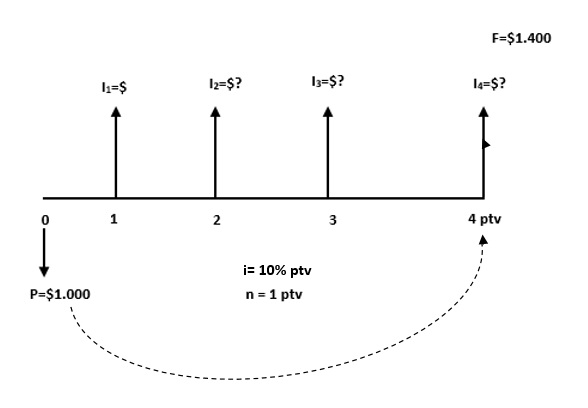
\includegraphics[height = 5.1 cm]{2_1}\\
	\end{center}
	
	\begin{table}[]
\centering
\label{my-label}
\begin{tabular}{|c|c|c|c|}
\hline
\begin{tabular}[c]{@{}c@{}}Periodo\\ {[}1{]}\end{tabular} & \begin{tabular}[c]{@{}c@{}}Capital Inicial (P) \\ {[}2{]}\end{tabular} & \begin{tabular}[c]{@{}c@{}}Interes simple (I)\\ {[}3{]}\end{tabular} & \begin{tabular}[c]{@{}c@{}}Capital final (F) \\ {[}4{]}\end{tabular} \\ \hline
0                                                         & \$1.000                                                                & 0                                                                    & \$1.000                                                              \\ \hline
1                                                         & \$1.000                                                                & \$100                                                                & \$1.100                                                              \\ \hline
2                                                         & \$1.000                                                                & \$100                                                                & \$1.200                                                              \\ \hline
3                                                         & \$1.000                                                                & \$100                                                                & \$1.300                                                              \\ \hline
4                                                         & \$1.000                                                                & \$100                                                                & \$1.400                                                              \\ \hline
\end{tabular}
\end{table}
	
    \item b. Declaración de variables:\\
	
	i= 10\% ptv\\
	n = $\frac{90\ d\acute{i}as}{90\ d\acute{i}as} = 1 ptv $\\
	
	\item c. Declaración de fórmulas:\\
	I=Pin \hspace{35 pt}  \textit{Interés monetario simple}\\
	
	\item d. Desarrollo matemático:\\
	I$_{1}$ = \$1.000x0,1x1\\
	I$_{1}$ = \$100\\
	
	I = 4x\$100\\
	I = \$400\\
	
	VF = P + 4I\\
	VF = \$1.400\\
	
	\item e. Respuesta\\
El valor de los intereses simples es:	I = \$400\\
	
\end{itemize}

B. Calculo de I al final del tiempo de la inversión capitalizando los intereses.\\


\begin{itemize}
	\item a. Diagrama de flujo de caja:
	
	\begin{center}
		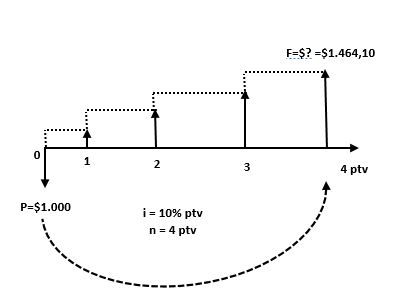
\includegraphics[height = 5.1 cm]{2_2}\\
	\end{center}
	
	\item b. Declaración de variables:\\
	
	i = 10\% ptv\\
	t = 360 días\\
	n = $\frac{360\ dias}{90\ dias} = 4 ptv$ \\
	
	\item c. Declaración de fórmulas:\\
	I= Pin \hspace{35 pt}  \textit{Interés monetario simple}\\
	Calculando para n= 1 ptv y capitalizando los intereses.\\
	
	\item d. Desarrollo matemático:
	
    \begin{table}[]
\centering
\label{my-label}
\begin{tabular}{|c|c|c|c|}
\hline
\begin{tabular}[c]{@{}c@{}}Periodo\\ {[}1{]}\end{tabular} & \begin{tabular}[c]{@{}c@{}}Capital Inicial (P) \\ {[}2{]}\end{tabular} & \begin{tabular}[c]{@{}c@{}}Interes simple (I)\\ {[}3{]}\end{tabular} & \begin{tabular}[c]{@{}c@{}}Capital final (F ó S) \\ {[}4{]}\end{tabular} \\ \hline
0                                                         & \$1.000                                                                & 0                                                                    & \$1.000                                                                  \\ \hline
1                                                         & \$1.000                                                                & \$100                                                                & \$1.100                                                                  \\ \hline
2                                                         & \$1.100                                                                & \$110                                                                & \$1.210                                                                  \\ \hline
3                                                         & \$1.210                                                                & \$121                                                                & \$1.331                                                                  \\ \hline
4                                                         & \$1.331                                                                & \$133,10                                                             & \$1.464,10                                                               \\ \hline
\end{tabular}
\end{table}
	
	\item e. Respuesta:\\
	
	I= \$ 464,10\\
\end{itemize}

\textbf{Generalizando se tiene que:}\\

Algebráicamente se puede representar el resultado anterior de la siguiente forma:\\


Con lo que llegamos a concluir que la fórmula del interés compuesto es:

	$F = P(1+i)^n$ \hspace{35 pt} \textit{Valor futuro}\\ 

\begin{table}[]
\centering
\label{my-label}
\begin{tabular}{|c|c|c|c|}
\hline
\textbf{\begin{tabular}[c]{@{}c@{}}Período (n)\\ {[}1{]}\end{tabular}}    & \textbf{\begin{tabular}[c]{@{}c@{}}Capital inicial (P)\\ {[}2{]}\end{tabular}}                     & \textbf{\begin{tabular}[c]{@{}c@{}}Interés (I)\\ {[}3{]}\end{tabular}}                                  & \textbf{\begin{tabular}[c]{@{}c@{}}Capital final (F)\\ {[}4{]}\end{tabular}}                                                                                                                                                       \\ \hline
\begin{tabular}[c]{@{}c@{}}0\\ 1\\ 2\\ 3\\ 4\\ .\\ .\\ .\\ n\end{tabular} & \begin{tabular}[c]{@{}c@{}}0\\ P\\ P(1+i)\\ $P(1+i)^{2}$\\ $P(1+i)^{3}$\\ .\\ .\\ .\\ $P(1+i)^{n-1}$\end{tabular} & \begin{tabular}[c]{@{}c@{}}0\\ Pi\\ P(1+i)i\\ $P(1+i)^{2}i$\\ $P(1+i)^{3}i$\\ .\\ .\\ .\\ $P(1+i)^{n-1}i$\end{tabular} & \begin{tabular}[c]{@{}c@{}}$F_{0}$ = P\\ $F_{1}$ = P + Pi = P(1+i)\\ $F_{2}$ = P(1+i) + P(1+i)i = $P(1+i)^{2}$\\ $F_{3}$ = $P(1+i)^{2}$ +$P(1+i)^{2}i$ = $P(1+i)^{3}$\\ $F_{4}$ = $P(1+i)^{3} + P(1+i)^{3}i = P(1+i)^{4}$\\ .\\ .\\ .\\ $F_{n} = P(1+i)^{n-1} + P(1+i)^{n-1}i = P(1+i)^{n}$\end{tabular} \\ \hline
\end{tabular}
\end{table}

\textbf{Volviendo al ejemplo 1:}\\

$F = P(1+i)^n$\\ 
$F = \$1.000 (1+0,1)^4$\\
$F = \$1.460,10$\\

C. ¿A qué tasa de interés periódica año vencido [$i_{2}$] es equivalente la tasa de interés del 10\% periódica trimestre vencido [$i_{1}$], del ejemplo anterior? Y calcule la tasa efectiva anual vencido de referencia.\\

\begin{itemize}
	\item a. Diagrama de flujo de caja:\\
	\begin{center}
		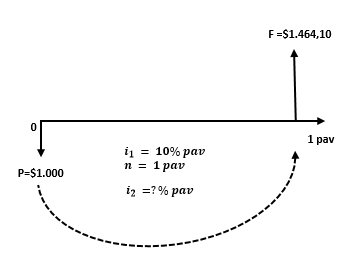
\includegraphics[height = 5.5 cm]{2_5}\\
	\end{center}
	
	\item b. Declaración de variables:\\
	
	i = ? \% pav\\
	t = 360 días\\
	P = \$1.000\\
	F = \$1.464,10\\
	n = $\frac{360 d\acute{i}as}{360 d\acute{i}as}$ = 1 pav\\
	
	\item c. Declaración de fórmulas:\\
	
	$VF = P(1+i)^n$ \hspace{35 pt} \textit{Valor futuro}
	
	\item d. Desarrollo matemático:\\
	
	\$1.464,10 = $\$1.000(1+i)^1$ \hspace{35 pt} \textit{Ecuación de valor}\\
	
	$\frac{\$1.464,10}{\$1.000} - 1 = i$\\
	
	i = 0,4641 pav\\
	
	\item e. Respuesta:\\
	
	i=46,41\%  pav\\
	j = im Tasa nominal anual\\
    $j = 46,41$ \%$ x 1 $pav $= 46,41$\ naav\Leftrightarrow  $46,41$\% EA\ 
	
	\textbf{Equivalente a:}\\
	j = i  m\\
	j = 10\% ptv x 4 ptv = 40\% natv\\
	j = 40\% natv\\
	
	\textbf{IMPORTANTE:} $40\% natv \equiv 46,4\% naav \equiv 46,4\% EA$\\
	
\end{itemize}

\textbf{Equivalencias de tasa de interés de 40\% natv con 46\% EA:}\\

%\usepackage{multirow}
\begin{table}[]
\centering
\label{my-label}
\begin{tabular}{|c|c|c|c|}
\hline
\textbf{Período trimestral} & \textbf{Capital} & \textbf{Interés} & \textbf{Tasa nominal}                            \\ \hline
0                           & \$100,0          & \$0,0            & \multirow{5}{*}{\textit{\textbf{j = 40\% natv}}} \\ \cline{1-3}
1                           & \$110,0          & \$10,0           &                                                  \\ \cline{1-3}
2                           & \$121,0          & \$11,0           &                                                  \\ \cline{1-3}
3                           & \$133,1          & \$12,1           &                                                  \\ \cline{1-3}
4                           & \textbf{\$146,4} & \$13,3           &                                                  \\ \hline
\end{tabular}
\end{table}

% \usepackage{multirow}
\begin{table}[]
\centering
\label{my-label}
\begin{tabular}{|c|c|c|c|}
\hline
\textbf{Período anual} & \textbf{Capital} & \textbf{Interés} & \textbf{\begin{tabular}[c]{@{}c@{}}Tasa nominal \equiv EA \\ \equiv Efectiva anual\end{tabular}} \\ \hline
0                      & \$100,0          & \$0,0            & \multirow{2}{*}{\textit{\textbf{j = 46,4\% naav}}}                                     \\ \cline{1-3}
1                      & \$146,4          & \$46,4           &                                                                                        \\ \hline
\end{tabular}
\end{table}

\section{Tasa de interés periódica (i)}

Es la expresión porcentual del interés aplicada a un capital en un período (por ejemplo diario, mensual, bimestral, trimestral, semestral, anual, bianual, etc..). Se representa por i.\\

\textbf{Tasa de interés nominal anual [j]}\\

Corresponde a la anualización de tasa periódica (i):\\

j = im ; En donde m = número de períodos de la tasa periódica.\\

$i = \frac{j}{m}$ \hspace{2 cm} \\

\textbf{Del ejemplo 1:}\\

i = 10\%  ptv\\
m = 4 ptv\\
j = i  m\\
j = 10\% x 4 ptv\\
j = 40\% natv\\

\textbf{Ejemplo 2}\\

Calcular la tasa periódica semestral vencida a partir del 28\% nominal anual semestre vencido. \\
\begin{itemize}
	
	\item a. Declaración de variables:\\
	
	j = 28\% nasv\\
	i = ?\% psv\\
	
	\item b. Declaración de fórmulas:\\
	
	j = im  \hspace{35 pt} \textit{Tasa de interés nominal}
	
	\item c. Desarrollo matemático:\\
	
	$i = \frac{28\%}{2} psv = 14\% $ psv\\
	
	\item e. Respuesta:\\
	
	i = 14\% psv\\
	
\end{itemize}

\textbf{Ejemplo 3}\\

Se invierte \$200.000 en un depósito a término fijo de 6 meses en un banco que paga el 28,8\% namv determinar el monto de la entrega al vencimiento.\\

\begin{itemize}
	\item a. Diagrama de flujo de caja:\\
	
	\begin{center}
		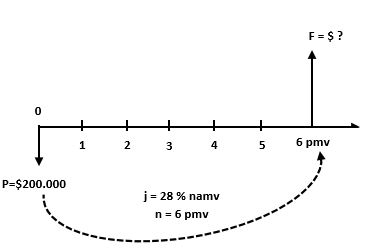
\includegraphics[height = 5.5 cm]{2_7}\\
	\end{center}
	
	\item b. Declaración de variables\\
	
	n = 6 pmv\\
	j = 28,8\% namv\\
	m = 12 pmv\\
	P = \$200.000\\
	F = \$?\\
	\item c.Declaración de fórmulas:\\
	
	$j = im$ \hspace{35 pt} \textit{Tasa de interés nominal anual vencida}\\
	
	$F = P(1+i)^n$ \hspace{35 pt} \textit{Valor futuro dado un valor presente}\\
	
	\item d. Desarrollo matemático:\\
	
	$i = \frac{28\%}{12} = 0,024$ pmv\\	
	$F = \$200.000 (1+0,024)^6$ \hspace{35 pt} \textit{Ecuación de valor} \\
	$F = \$230.584,30$\\
	
	\item e. Respuesta: \\
	
	$F = \$230.584,30$\\
	
\end{itemize}

\textbf{Ejemplo 4}\\

Una persona debe cancelar la suma de \$ 2'000.000 al cabo 18 meses. ¿Cuál debe ser el valor del ahorro que debe hacer hoy en una cuenta que paga el equivalente al 32\% nominal anual trimestre vencido para poder cancelar la deuda?\\

\begin{itemize}
	\item a. Diagrama de flujo de caja de la persona:\\
	\begin{center}
		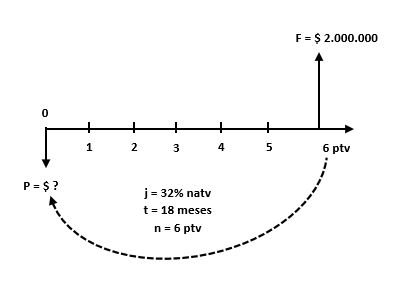
\includegraphics[height = 5.3 cm]{2_8}\\
	\end{center}
	
	\item b. Declaración de variables:\\
	
	t = 18 meses\\
	\\
	$n = \frac{18 meses}{3 meses}$ = 6 ptv\\
	\\
	j=32\% natv\\
	\\
	i=  $\frac{32\% natv}{4 ptv}$\\
	\\
	i = 8\% ptv\\
	\\
	F = \$ 2'000.000\\
	\\
	P = \$?\\
	
	\item c. Declaración de fórmulas:\\	
	F = $ P(1 + i)^n$ \hspace{35 pt} \textit{Valor futuro dado un valor presente}
	
	P = $\frac{F}{(1 + i)^{n}}$ \hspace{35 pt} \textit{Valor presente dado un valor futuro}\\	
	\item d. Desarrollo matemático:\\
	
	P = $\frac{\$2'000.000}{(1 + 0,08)^6}$ \hspace{35 pt} \textit{Ecuación de valor}\\
	
	P =  \$1'260.339,25\\
	
	\item e. Respuesta:\\
	
	P =  \$1'260.339,25\\ 
\end{itemize}

\textbf{Ejemplo 5}\\

¿A qué tasa nominal anual mes vencido se triplica un capital en $2^{\frac{1}{2}}$ años?\\

\begin{itemize}
	\item a. Diagrama de flujo de caja:\\
	\begin{center}
		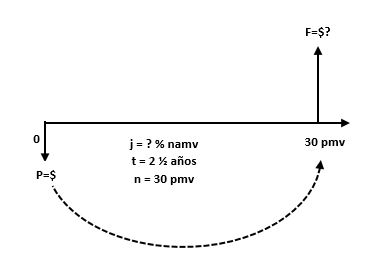
\includegraphics[height = 5.3 cm]{2_9}\\
	\end{center}
	
	\item b.Declaración de variables\\
	
	t = $2^{\frac{1}{2}}$ años\\
	n = 30 pmv\\
	j = ? \% namv \\
	m = 12 pmv\\
	P = ? \\
	F = ? \\
	
	\item c. Declaración de fórmulas:\\
	
	F = $ P(1 + i)^n$ \hspace{35 pt} \textit{Valor futuro}\\
	
	j = im \hspace{35 pt} \textit{Tasa nominal anual}\\
	
	\item d. Desarrollo matemático:\\
	
	\$3 = \$1 $(1 + i)^{30}$ \hspace{35 pt} \textit{Ecuación de valor}\\
	
	$\frac{\$3}{\$1}^{\frac{1}{30}} - 1$ = i\\
	
	i = 0,0373 pmv\\
	i = 3,73\% pmv\\
	
	Equivalente a:\\
	
	j = 3,73\%pmv x 12\%pmv\\
	j = 44,76\% namv\\
	
	\item e. Respuesta:
	
	j = 44,76\% namv\\
	
\end{itemize}

\textbf{Ejemplo 6}

¿En cuánto tiempo se duplica un capital a una tasa del 24\% nominal anual mes vencido?\\

\begin{itemize}
	\item a. Diagrama de flujo de caja:\\
	\begin{center}
		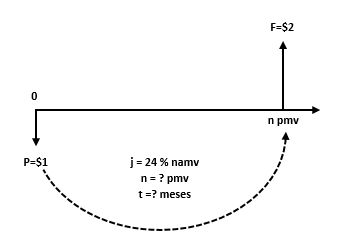
\includegraphics[height = 5.3 cm]{2_10}\\
	\end{center}
	\item b. Declaración de variables:\\
	
	j = 24\% namv\\ % \hspace{1 cm} i = 2\% pmv\\
	n = ? pmv\\
	P = 1\$\\
	F = 2\$\\
	t = ?\$ meses\\
	
	\item c. Declaración de fórmulas:\\
	
	j = im \hspace{35 pt} \textit{Tasa nominal anual}\\
	
	F = $ P(1 + i)^n$ \hspace{35 pt} \textit{Valor futuro}\\
	
	\item d. Desarrollo matemático:\\
	
	$i= \frac{0,24 namv}{12 pmv}$\\

	i= 0,02 pmv\\
	
	\$2 = \$1 $(1+0,02)^n$ \hspace{35 pt} \textit{Ecuación de valor}\\
	log2 = nlog(1,02)\\
	
	n = $\frac{log2}{log(1,02)} = 35$ pmv\\
	
	$n = 35 pmv \equiv t=35 meses$\\
	
	
	\item e. Respuesta:\\
	
	n = 35 pmv\\
	t = 35 meses\\
	
\end{itemize}

\section{Equivalencia de tasas ($i_{1} \equiv i_{2}$)}

Tasas equivalentes de interés son aquellas que teniendo diferente periodicidad y/o modalidad de liquidación de intereses producen el mismo monto al final o al comienzo del flujo.\\

\textbf{Ejemplo 7}\\

¿A qué tasa de interés periódica semestre vencido se debe invertir un capital para que el valor al vencimiento de un año sea igual a la misma inversión a una tasa periódica del 10\% periodo trimestre vencido?¿Cuál es el valor final  de \$100 al 10\% ptv= ? 
\begin{itemize}
	\item a. Diagrama de flujo de caja:
	
	\begin{center}
		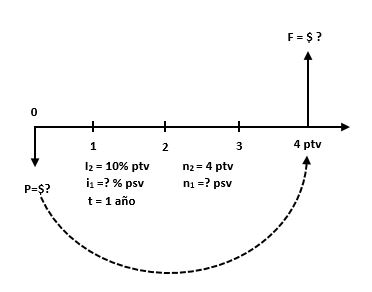
\includegraphics[height = 5.3 cm]{2_11}\\
	\end{center}
	
	\item b. Declaración de variables:\\ \\
	
	
	
	$i_{2}$ = 10\% ptv \\
	$m_{2}$ = 4 ptv\\
	t = 1 año\\
	$i_{1}$ = ? \% psv \\
	$m_{1}$ = 2 psv\\
	P = \$100\\
	F = \$?\\
	 
	
	\item c. Declaración de fórmulas:\\
	
	
	$(1+i_{1})^{m_{1}}$ = $(1+i_{2})^{m_{2}}$ \hspace{35 pt} \textit{Equivalencia de tasas}\\
    F = $ P(1 + i)^n$ \hspace{70 pt} \textit{Valor futuro dado un valor presente}\\
	\item d. Desarrollo matemático:\\
	
    $(1+i_{1})^{2} = (1+0,1)^{4}$\\
    
    $i_{1} = 21$ \% psv \\  
	 	
	
	   F= $\$100 (1 + 0,1)^{4}$ \\
       F = \$146,41
       
 \item e. Respuesta:\\
	
	i$_{1}$ = 21 \% psv \\
	F = \$146,41 \\\\
	
	
\end{itemize}

\textbf{Ejemplo 8}\\

Dado el 5\% período bimestre vencido, calcular una tasa periódica trimestral vencido.\\

\begin{itemize}
	\item a. Declaración de variables:\\
	
	$i_{1}$ = 5\% pbv\\
	$m_{1}$ = 6 pbv\\
	$i_{2}$ = ?\% ptv\\
	$m_{2}$ = 4 ptv\\
	
	\item b. Declaración de fórmulas:\\
	
	$(1+i_1)^{m_1} = (1+i_2)^{m_2}$ \hspace{35 pt} \textit{Equivalencia de tasas}\\
	
	\item c. Desarrollo matemático:\\
	
	Reemplazando: $(1+0,05)^{6} = (1+i_{2})^{4}$ \hspace{35 pt} \textit{Ecuación de valor}\\
	
	\item d. Respuesta:\\
	
	$i_{2} = 7,59\% ptv  \equiv j_{2} = 30,37$\% natv\\
	
	
	\item f. Justificación:\\
	
	\begin{table}[H]
\centering
\begin{tabular}{|c|c|}
\hline
$i_{1} = 5$\% pbv    & $$\equiv j_{1} =  5x6 = 30$$\% nabv\\ \hline
$i_{2} = 7,59$\% ptv & $$\equiv j_{2} = 30,37$$\% natv\\ \hline
\end{tabular}
\end{table}
	
	En tasas nominales anuales vencidas a medida que aumenta el tiempo del período, aumenta el valor absoluto de la tasa.\\
	
\end{itemize}

\textbf{Ejemplo 9}\\

Dado el 36\% nominal anual mes vencido, hallar una tasa nominal anual semestre equivalente.\\

\begin{itemize}
	\item a. Diagrama de equivalencia de tasas:\\
	\begin{center}
		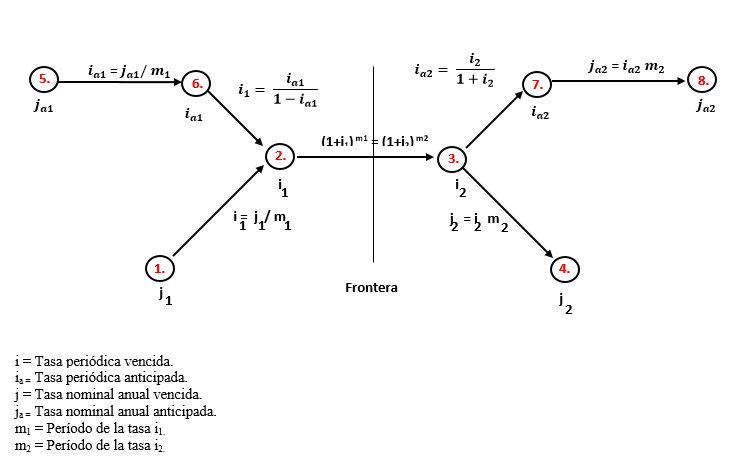
\includegraphics[height = 9.0 cm]{general}\\
	\end{center}
	
	\item b. Declaración de variables:\\
	
	${j_1}$ = 36 \% namv \\	
	${i_1}$ = $\frac{36\% namv}{12 pmv} = 3\% $ pmv\\
	
	$m_{1} $= 12 pmv \\
	${j_2}$ = ? \% nasv\\
	$m_{2} $= 2 psv\\
	
	
	\item c. Declaración de fórmulas:\\
	
	$(1+i)^{m_1} = (1+i)^{m_2}$ \hspace{35 pt} \textit{Equivalencia de tasas}\\
	$j_{1} = i m$\hspace{35 pt} \textit{Tasa nominal anual }\\
	
	\item d. Desarrollo matemático:\\
	Reemplazando\\
	$(1+0,03)^{12} = (1+i_2)^{2}$\\
	$i_{2}$ = 19,405229653\% psv\\
	$j_{2} = i_{2} x m_{2}$\\
	$j_{2} = 19,405229653$\%nasv x 2 psv\\
    $j_{2} = 38,81$\%nasv\\
	\item e. Respuesta\\
	
	$j_{2}$ = 38,81\%nasv\\
\end{itemize}

La solución del problema anterior implicó partir del punto 1 y llegar al punto 4, pasando por los puntos intermedios 2 y 3 De acuerdo con la siguiente gráfica:

\begin{center}
		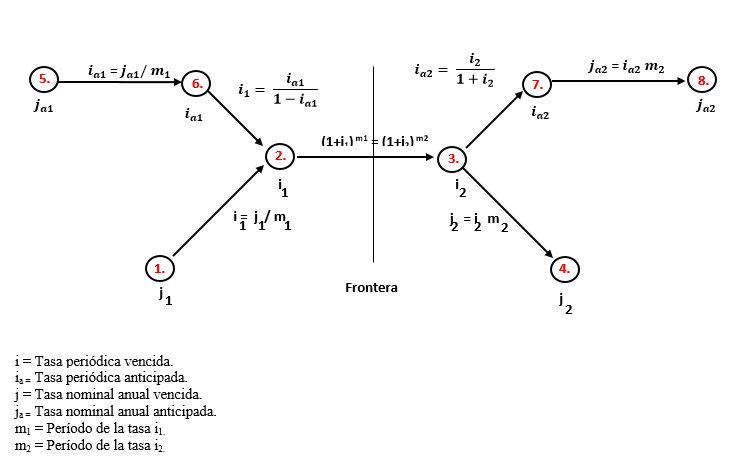
\includegraphics[height = 9.0 cm]{general}\\
\end{center}

En el punto 1 $j_{1}$ = 36\% nasv, en el punto 2 $i_{1} = 3\%$ pmv, en el punto 3 $i_{2} = 19,052$\% psv y en el punto 4 $j_{2} = 38,81\%$ nasv.\\

\textbf{Ejemplo 10}\\

Dado el i=2,5\% periódica mes vencido, hallar una tasa nominal anual trimestral vencida equivalente.\\

\begin{itemize}
	\item a. Diagrama de equivalencia de tasas:\\
	
	\begin{center}
	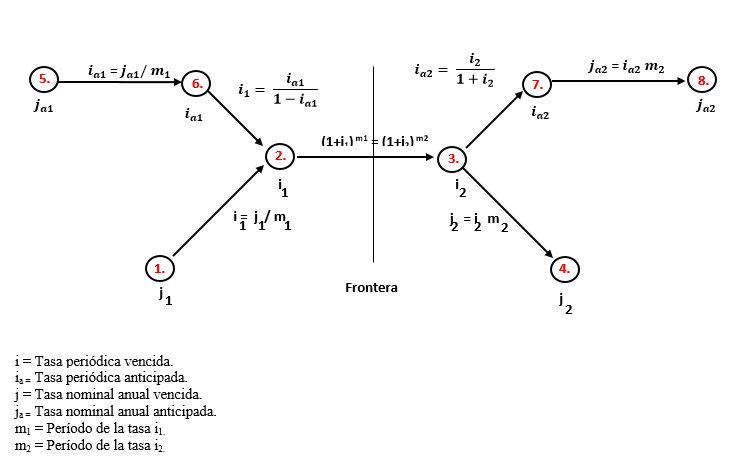
\includegraphics[height = 9.0 cm]{general}\\		
	\end{center}
	
	\item b. Declaración de variables:\\
	
	De la gráfica, se trata de pasar por los puntos 2, 3 y 4.\\
	
	$i_{1}$ = 2,5\% pmv\\
	$m_{1}$ = 12 pmv\\
	$i_{2}$ = ?\% ptv\\
	$m_{2}$ = 4 ptv\\
	
	
	\item c. Declaración de fórmulas:\\
	
	$(1+i)^{m_1} = (1+i)^{m_2}$ \hspace{35 pt} \textit{Equivalencia de tasas}\\
	$j_{2} = i_{2}$  m$_{2}$\hspace{35 pt} \textit{tasa nominal anual}\\
	
	\item d. Desarrollo matemático:\\
	$(1+0,025)^{12} = (1+i_{2})^{4}$\\
	$(1,025)^{\frac{12}{4}}-1 = i_{2}$ \\
	i$_{2}$ = 7,6890625\% ptv\\
	\\
	j$_{2}$ = 7,6890625\% ptv x 4 ptv \\
	
	\item e. Respuesta:\\
	
	j$_{2}$ = 30.756\% natv\\
\end{itemize}

\section{Tasa de interés nominal anual (j) y tasa efectiva anual (EA)}

Según la Superintendencia Financiera de Colombia, SuperFinanciera, la tasa de interés nominal anual es la tasa que el emisor paga al inversionista por un título valor. Las tasas nominales anuales corresponden a la anualización de una tasa periódica, que puede ser diaria, mensual, trimestral, semestral, anual o cualquier otro que se establezca. De igual forma, pueden tener modalidad vencida o anticipada para la liquidación de intereses.\\

\textbf{Tasa de interés efectiva anual:} La tasa de interés efectiva anual, es el instrumento apropiado para medir y comparar, el rendimiento de distintas alternativas de inversión según la Superintendencia Financiera. Según el profesor Javier Serrano, en el libro “Matemáticas financieras y evaluación de proyectos”, la tasa de interés efectiva anual corresponde a aquella tasa de interés que paga de una sola vez al final del año, permite acumular la misma cantidad de dinero que una tasa nominal pagado por período vencido cuando los intereses se reinvierte.\\

Para calcular la tasa efectiva anual, se parte de la fórmula de equivalencia de tasas en donde el periodo es anual vencido.\\ 

	$(1+i)^{m_1} = (1+i)^{m_2}$,
en donde i$_{1}$ = tasa periódica, que anualizada (j$_{1}$) es equivalente a la tasa efectiva anual, para un m$_{1}$ = 1 pav.\\ \\ \\


\textbf{Ejemplo 11}

¿Cuál es la tasa efectiva anual de una tasa del 36\% nominal anual mes vencido?\\

\begin{itemize}
    \item a. Diagrama de equivalencia de tasas:\\
	
	\begin{center}
	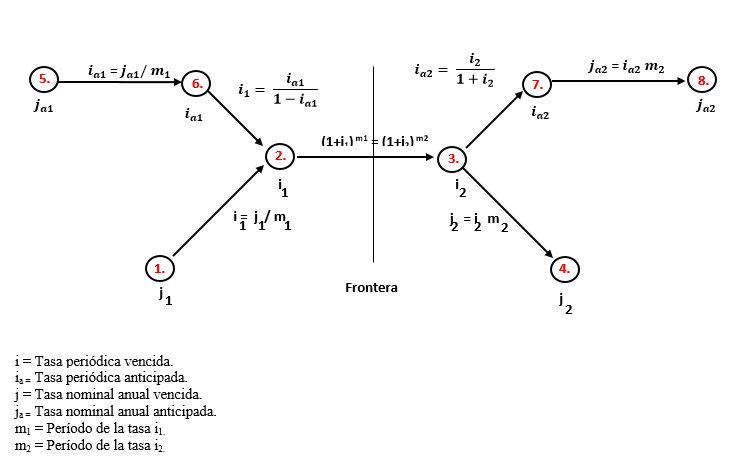
\includegraphics[height = 9.0 cm]{general}\\		
	\end{center}
	
	\item b. Declaración de variables:\\
	$j_{1}$ = 36\% namv \\ 
	m$_{1}$= 12 pmv \\
	$j_{2}$ = ?\% EA\\
	m$_{2}$= 1 pav \\
	\item c. Declaración de fórmulas:\\
		$(1+i)^{m_1} = (1+i)^{m_2}$  \hspace{35 pt} \textit{Equivalencia de tasas}\\
     j= i  m    \hspace{70 pt}\textit{Tasa nominal anual vencida}   \\
	
	\item d. Desarrollo matemático:\\
	
	i$_{2}$ = $\frac{36\%namv}{12 pmv }= 3\% pmv $\\ \\
	
		$(1+i)^{1} = (1+0,03)^{12}$ \\

i$_{2}$ = 42,675 \% pav\\
j$_{2} = 42,675 \% pav x 1 pav = 42,675 \% naav  \equiv
   42,675 \% EA$ \\
	
	\item e. Respuesta:\\

    j$_{2} = 42,675 \% pav\equiv
   42,675 \% EA$ \\
	

\end{itemize}


\textbf{Ejemplo 12}\\

¿Cuál es el interés efectivo anual equivalente a un $j=32\%$ nominal anual trimestre vencido?\\

\begin{itemize}
	\item a. Diagrama de equivalencia de tasas:\\
	
	\begin{center}
	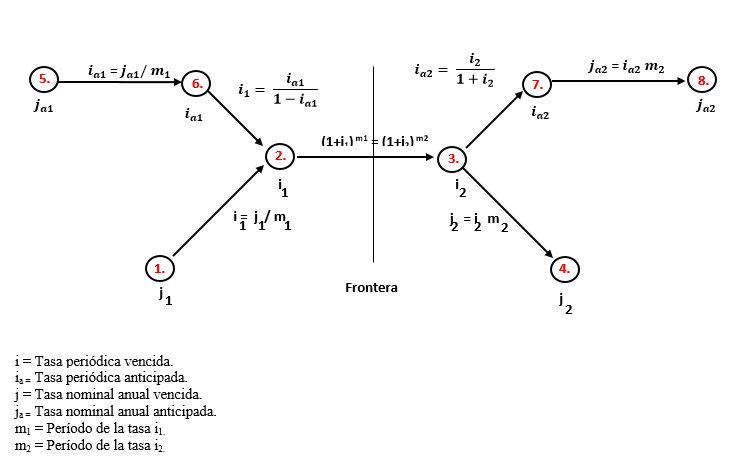
\includegraphics[height = 9.0 cm]{general}\\		
	\end{center}
	
	\item b. Declaración de variables:\\
	
%	Al año se tienen 4 trimestres de forma\\
	$j_{1} = 32$\% natv \Rightarrow $i_{1} = 8$\% ptv\\
	$m_{1}$ = 4 ptv\\	
	$j_{2} = ?\%\ EA$\\ 
	m$_{2}$ =  1 pav\\
	
	
	\item c. Declaración de fórmulas:\\
	$(1+i1)^{m_1} = (1+i2)^{m_2}$ \hspace{35 pt} \textit{Equivalencia de tasas}\\
	j = i m \hspace{35 pt} \textit{Tasa nominal  anual vencida}\\
	
	\item d. Desarrollo matemático\\
	$(1+0,08)^{4} = (1+i_{2})^{1}$\\
	$i_{2}$= 36.05\% pav \Rightarrow $j_{2} = 36$ \% $x 1$ pav $= 36$\% naav \equiv $36$\% EA\\
	
	\item e. Respuesta:\\
	$j_{2} = 36,05$ \% naav  \equiv $36,05$ \% EA\\
	
\end{itemize}

\textbf{Ejemplo 13}\\

¿ Cuál es la tasa efectiva anual equivalente al 36\% nominal anual semestre vencido?\\

\begin{itemize}
    \item a. Diagrama de equivalencia de tasas\\
    
	\item b. Declaración de variables:\\
	$j_{1} = 36$\%nasv \Rightarrow $i_{1} =$\frac{$36$\%nasv}{$2$} $= 18$\% psv \\
	$m_{1} = 2$ psv\\
	
   
    $j_{2}$ = ? \% EA \\
    $m_{2}$ = 1 pav \\
	
	\item c. Declaración de fórmulas:\\
	$(1+i)^{m_1} = (1+i)^{m_2}$ \hspace{35 pt} \textit{Equivalencia de tasas}\\
	j = i m \hspace{35 pt} \textit             {Tasa nominal anual}\\
	
	\item d. Desarrollo matemático:\\
	
		$(1+0,18)^{2} = (1+i_{2})^{1}$ \\
		$i_{2} = 0,39240$  pav\\
		$j_{2} = 39,24$\% $x1$ pav $= 39,24$\% naav \equiv $39,24$\% EA
	
	\item e. Respuesta:\\
	
	$j_{2}$ = 39, 224 \% EA\\
	
\end{itemize}


\textbf{Ejemplo 14}\\

Suponga que una cuenta de ahorros de un banco le paga una tasa efectiva anual del 19\%, ¿Cuál sería la tasa periódica diaria? Asuma un año de 365 días.\\

\begin{itemize}
    \item a. Diagrama de equivalencia de tasas:\\
\begin{center}
	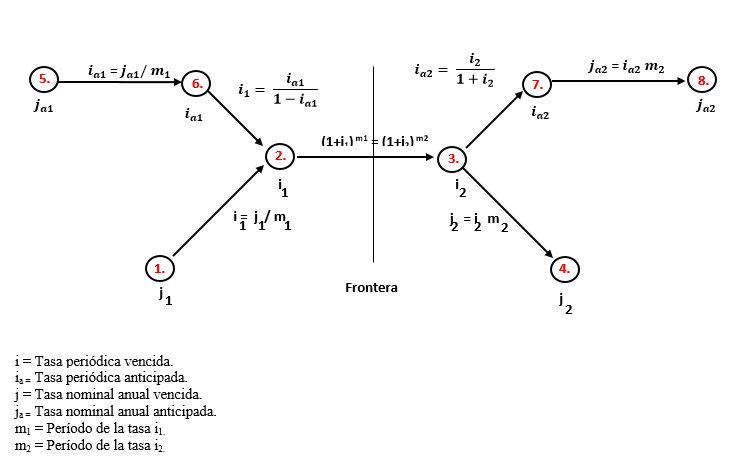
\includegraphics[height = 9.0 cm]{general}\\
\end{center}   
	\item b. Declaración de variables:\\
	
	
	$j_{1} = 19$\% EA \equiv $19$\% naav \Rightarrow $i_{1} = 19$\% pav\\
	m$_{1}$= 1 pav\\
    $i_{2}$ = ? \% pdv \\
    $m_{2}$ = 365 pdv \\
	
	\item c. Declaración de fórmulas:\\
	 $(1+i)^{m1} = (1+i)^{m2}$ \hspace{70 pt}\textit{Equivalencia de tasas:}\\
	j = i m \hspace{15 pt}\textit{Tasa nominal anual}\\
	
	\item d. Desarrollo matemático:\\
	
   
    $(1+0,19)^{1} = (1+i2)^{365}$ \\
	Despejando se obtiene:\\
	
	$i = 1,19 ^{\frac{1}{365}} = 0,00498$ pdv \Rightarrow 0,498\% pdv\\
	
	\item e. Respuesta:\\
	
	i$_{2}$ = 0,498\% pdv\\
	j$_{2}$ = 0,498\% pdv x 365 pdv = 181,77\% nadv\\
	
\end{itemize}



\textbf{Ejemplo 15}\\

¿Cuál es la tasa de interés nominal anual trimestre vencido, equivalente al 18\% nominal anual mes vencido?

\begin{itemize}
    \item a. Diagrama de equivalencia de tasas:\\
\begin{center}
	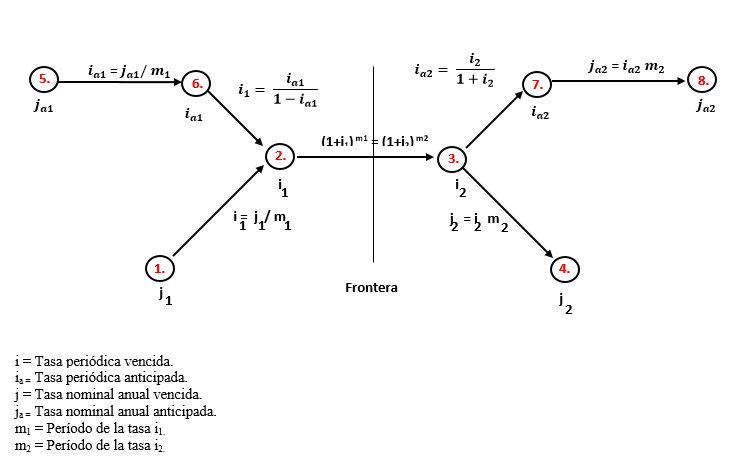
\includegraphics[height = 9.0 cm]{general}\\
\end{center}    
	\item b. Declaración de variables: \\
	$j_{1} = 18$\% namv \Rightarrow $:{i1} =$ \frac{$18$\% namv}{$12$ pmv} $= 1,5$\% pmv\\
	$m_{1}$ = 12 pmv \\
	$j_{2}$ = ? \% natv \\
    $m_{2}$ = 4 ptv \\
   
	

	\item b. Declaración de fórmulas:\\
	
	$(1+i)^{m_1} = (1+i)^{m_2}$\hspace{35 pt}\textit{Equivalencia de tasas}\\
	j = i m \hspace{90 pt}\textit{Tasa nominal anual}\\
	
	\item c. Desarrollo matemático:\\
	
	Primero se calcula el interés mes vencido equivalente a un interés nominal mes vencido del 18\% namv:\\
	
	i$_{1}$= 18\% namv / 12 = 1,5\% pmv
	$(1+0.015)^{12} = (1+i_{2})^{4}$ \\
	
	Despejando:\\
	
	$i_{2} = (1,015)^{\frac{12}{4}} - 1 = 0,04567$ ptv\\
	
	Por lo tanto el interés nominal anual que, pagadero trimestre vencido, es equivalente a un interés del 18\% nominal anual pagadero mes vencido, sería igual a:\\
	
	j = 4 * $i_{2} = 4 * 0,0456 = 0,18271 = 18,271$\% natv\\
	
	Por ello, un interés nominal anual del 18,271\% natv, es equivalente a un interés del 18\% namv.\\
	
	$j_{tv} $=  $18,271$\% natv \equiv 18\% namv\\
	
	\item e. Respuesta:\\
	
	j= 18,271\% natv\\
	
\end{itemize}

\section{Relación entre una tasa de interés anticipada(i$_{a}$) y una tasa vencida(i)}

Para $n = 1$, se tiene 
$i = \frac{I}{P}$ \\
Si \\
$I = F  d$ \\
y \\
$P = F (1 -d)$, \hspace{35 pt}\textit{Tasa nominal anual}\\
remplazando en i \\
$i = \frac {F d} {F (1-d)}$,\hspace{35 pt}\textit{Tasa nominal anual.}\\
factorizando F, tenemos: \\
$i = \frac{d}{(1 - d)}$ \hspace{35 pt}\textit{Tasa nominal anual.}\\
Remplazando $d = i_{a} $,tenemos: \\
$i = \frac{ia}{(1 - ia)}$, \hspace{35 pt}\textit{Tasa nominal anual.}\\
despejando $i_{a}$: \\
$i_{a} = \frac{i}{(1+i)}$ \\

$i = \frac{I}{P} = \frac{F d}{F(1-d)}$\\

$i = \frac{d}{1-d}$\\

Reemplazando d = $i_{a}$\\

Despejando $i_{a}$ = ?\\

$i_{a} = \frac{i}{1+i}$  Tasa periódica anticipada\\

Tasa nominal anual anticipada\\

$j_{a} = i_{a}  m$\\


\section{Gráfica de equivalencia de tasas}

Los puntos que se han colocado del 1 al 8 solo sirven de identificación y no es más que una ampliación de la gráfica mostrada en el ejemplo 9.\\

\begin{center}
	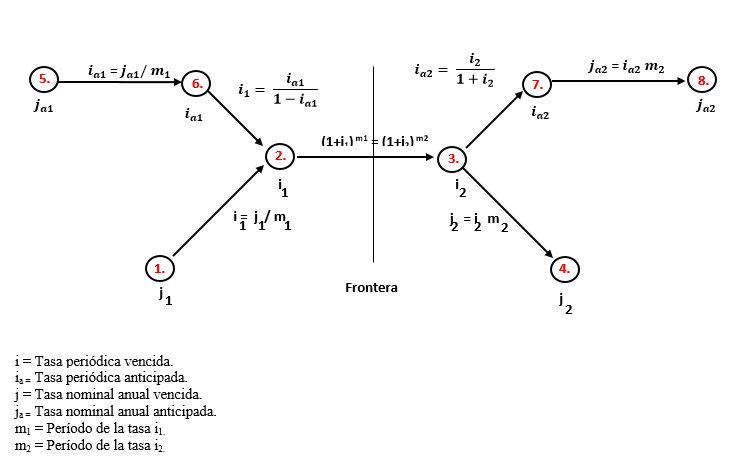
\includegraphics[height = 9.0 cm]{general}\\
\end{center}


\textbf{Observación:} La gráfica equivalencia de tasas, siempre se debe comenzar de un punto de la izquierda y seguir la trayectoria hasta llegar a otro punto situado en la parte derecha.\\

\textbf{Ejemplo 16}\\

Dado el 36\% nominal anual mes vencido hallar:\\

a. Una tasa efectiva anual. \\ 
b. Una tasa nominal anual semestre vencido. \\
c. Una tasa periódica bimensual vencida. \\
d. Una tasa nominal periódica semestre anticipado. \\

a. Diagrama de equivalencia de tasas:\\
\begin{center}
	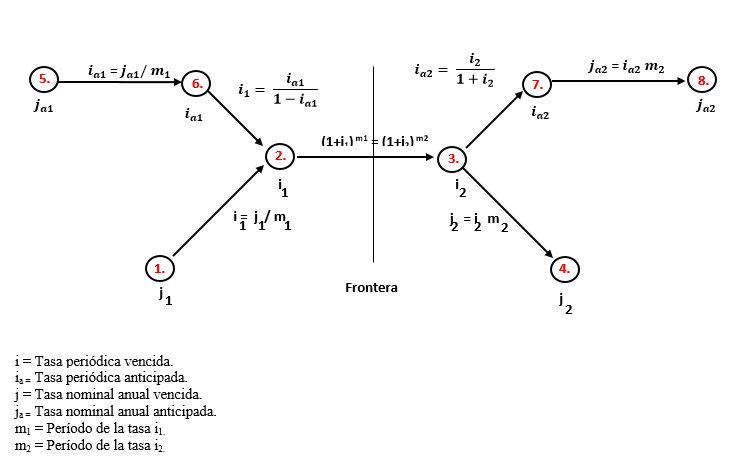
\includegraphics[height = 9.0 cm]{general}\\
\end{center}

\textbf{Solución}\\

\textbf{Parte a.}\\
En el punto (1). j = 36\%namv\\
En el punto (2) $i=\frac{j}{m} = \frac{36\%namv}{12 pmv} = 3$\% pmv\\
Para el paso (2) a (3) planteamos la ecuación $(1+0,03)^{12}= (1+i_{2})^1$ obsérvese que el primer paréntesis se eleva a la potencia 12 porque la tasa del 3\% tiene periodicidad mensual y en un año hay 12 períodos; el segundo paréntesis se eleva a la potencia 1 por que la tasa debe tener una periodicidad anual, es decir es una tasa periodica año vencido; al despejar $i_{2}$ de esta ecuación se tiene:\\

$i_{2}$ = 42,576088685\%  \\j = 42,576\%x1 pav\\
$j = 42,576$\%naav $$\equiv  42,576$$\% EA\\

\textbf{Parte b}.\\
El punto de partida es el punto (1) y el punto de llegada debe ser el punto (4).\\
En el punto (1)  j=36\%namv\\
En el punto (2)  $i=\frac{j}{m} = \frac{36\% namv}{12 pmv} = 3\%$ pmv\\
Para el paso (2) a (3) planteamos la ecuación $(1+i_{1})^{m_{1}}= (1+i_{2})^{m_{2}}$\\
Remplazando $m_{1}$ = 12 pmv y m$_{2}$ = 2 pmv\\

$(1 + 0,03)^{12} = (1 + i2)^2$\\

Obsérvese que el segundo paréntesis se elevó a la potencia 2 por que la tasa debe tener una periodicidad semestral y en un año hay 2 semestres: Al despejar $i_{2}$ de esta ecuación se obtendrá: $i_{2}$ = 19,405229653\% psv.\\


Para el paso de (3) a (4) simplemente multiplicamos el resultado anterior por 2 porque en el lado derecho de la frontera los períodos son semestres y así tenemos:\\ 

j = 19,405229653\%psv\\ x 2 = 38.81\%psv\\
j = 38,81\% nasv\\

\textbf{Parte c}.\\

El punto de partida es el punto (1) y el punto de llegada es el punto 3 del diagrama de conversión de tasas.\\

En los puntos 1 y 2 se tienen los mismos resultados de la parte a o de la parte b por consiguiente en punto 2 i=3\% pmv\\

En el punto 2 al 3 implica el planteo de la ecuación:\\

$(1+i_{1})^{m_{1}} =(1+i_{2})^{m_{2}}$\\
$(1 + 0,03)^{12} = (1 + i)^6$\\

Obsérvese que el exponente del segundo paréntesis debe ser 6 por que en la parte derecha de la frontera los períodos son bimestres y en un año hay 6 bimestres. Al despejar se obtiene:\\ 
i=6,09\% pbv\\

j = 6,09 x 6 = 36,54 nabv\\

\textbf{Parte d.}\\

El punto inicial es el 1- y el punto de llegada debe ser el punto (8).\\ 
En los puntos 1 y 2 los resultados son los mismos que los mostrados en las partes a b o c.\\
El punto 2 al 3 implica planteamiento de la ecuación\\ 

$(1+i_{1})^{m_{1}} =(1+i_{2})^{m_{2}}$\\
$(1+0,03)^{12} = (1+ i2)^2$\\

Y al despejar se tiene que: i2 = 19,405229653 \% psv \\ 
El paso del 3 al 7 implica plantear la ecuación:\\ 

$i_{a} = \frac{i}{1+i}$ \hspace{35 pt} \textit{Tasa periódica anticipada}\\

$\frac{0,19405229653}{1+0,19405229653}$ = 16,2515743317\% psa\\

El paso (7) al (8) implica multiplicar el resultado anterior por 2 y se tiene:\\

$j_{a} = 16,2515743317 x 2 = 32,5\% nasa$\\

Resumen:\\

% \usepackage{multirow}
\begin{table}[]
\centering
\caption{My caption}
\label{my-label}
\begin{tabular}{|c|c|c|c|c|}
\hline
\multicolumn{4}{|c|}{\textbf{\begin{tabular}[c]{@{}c@{}}Equivalencia de tasas nominales anuales (j) con \\ periodicidad y modalidad diferente\end{tabular}}} & \textbf{\%EA}                                                                                 \\ \hline
                                           & Valor                              & Período                        & \textbf{Modalidad}                        & \multirow{6}{*}{\begin{tabular}[c]{@{}c@{}}j = 42,576\% naav\\ \\ = 42,576\% EA\end{tabular}} \\ \cline{1-4}
\multirow{2}{*}{d}                         & 32,5\% na                          & s                              & a                                         &                                                                                               \\ \cline{2-4}
                                           & 36,0\% na                          & m                              & v                                         &                                                                                               \\ \cline{1-4}
c                                          & 36,54\% na                         & b                              & v                                         &                                                                                               \\ \cline{1-4}
b                                          & 38,81\% na                         & s                              & v                                         &                                                                                               \\ \cline{1-4}
a                                          & 42,576\% na                        & a                              & v                                         &                                                                                               \\ \hline
\end{tabular}
\end{table}

\textbf{Ejemplo 17}\\

¿Cuál es la tasa periodica mes anticipada equivalente a una tasa 30\% nominal anual trimestre anticipada?\\

a. Diagrama de equivalencia de tasas:\\

\begin{center}
		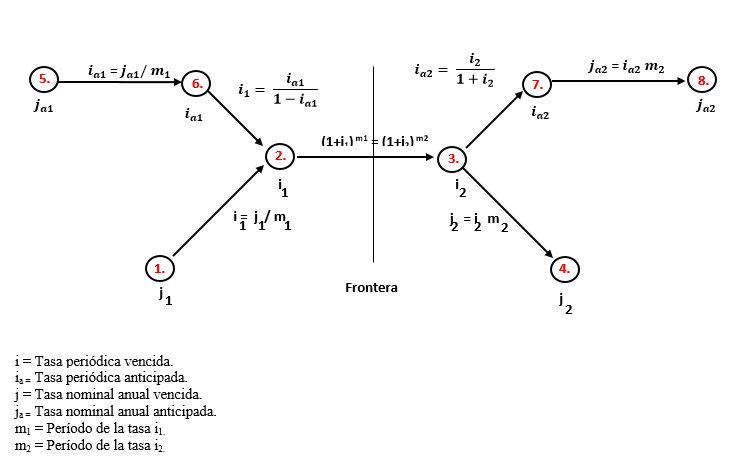
\includegraphics[height = 9.0cm]{general}\\
\end{center}

\textbf{Solución:}

Nos situamos en el punto 5 como punto de partida que corresponde a una tasa anual trimestre anticipado y nuestro destino final será el punto 7 que corresponde a una tasa periódica mensual anticipada.\\

En el punto 5 $ j_{a} =30\%$ nata\\
En el punto 6 $i = \frac{i_{a}}{1-i_{a}} = \frac{0,075}{1-0,075}$ = 8,108108\% ptv\\

El paso de 2 a 3 implica el planteo de la ecuación.\\


$(1+i_{1})^{m_{1}} =(1+i_{2})^{m_{2}}$ \hspace{35 pt} \textit{Equivalencia de tasas}\\
$(1+0,08108108)^4 = (1 + i2)^{12}$\\

Obsérvese que en el primer paréntesis quedo elevado a la potencia 4 por que la tasa es periódica trimestre vencido y el segundo paréntesis quedó elevado a la potencia 12 porque los nuevos períodos deben ser mes vencido así:\\

i2 = 2,632779103\% pmv\\

El paso 3 al 7 implica el planteo de la ecuación\\ 


$i_{a} = \frac{i}{1-i}$ \hspace{35 pt} \textit{tasa periódica anticipada}\\

i$_{a}$ = $\frac{0,0263277910}{1+0,0263277910}$ = 2,565\% pma\\

$j_{a} $= 30\% nama\\

\textbf{Ejemplo 18}\\

¿Cuál es la tasa efectiva anual equivalente a una tasa 28\% nominal (258 días) vencido? Asuma el año de 365 días.\\

a. Diagrama de equivalencia de tasas:

\begin{center}
	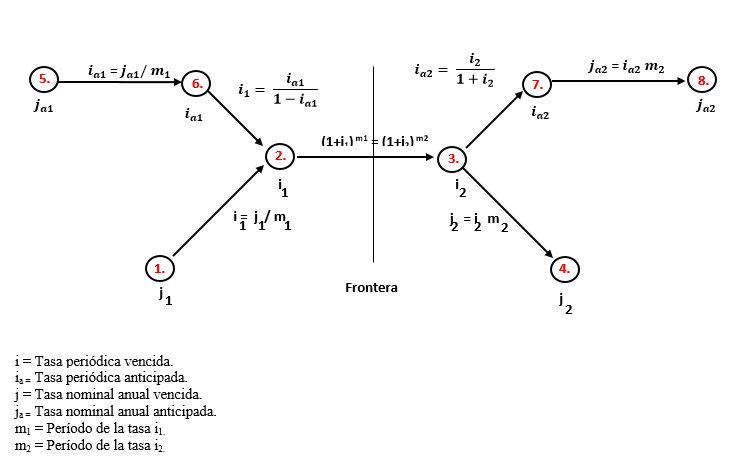
\includegraphics[height = 9.0 cm]{general}\\
\end{center}

\textbf{Solución:}\\

Iniciamos en el punto 1 y vamos al punto 3.\\
En el punto 1 j = n(258)dv\\

Para llegar al punto 2 sabemos que i = $\frac{j}{m}$ como el período tiene 258 días, entonces en un año habrá $\frac{365}{258}$ = 1.414729 períodos vencidos y al reemplazar en la formula anterior tenemos:\\

$i=\frac{0,28}{1.414729} = 0.197918 = 19.7918\%$ p258dv\\

i = 19.7918\% p258dv


Para el paso de 2. a 3.\\

$(1 + i_{1})^{m_{1}} = (1+ i_{2})^{m_{2}}$ \hspace{35 pt}\textit{Equivalencia de tasas}\\
$(1 + 0.197918)^{\frac{365}{258}} = (1 + i)^1$ \\
Despejando se tiene que i=29,10797\% pav\\
j=im\\
=29,10797\%x1 pav\\
$j=29,10797\%naav \equiv 29,10797$\% EA\\

\textbf{Ejemplo 19}\\

¿Cuál es la tasa nominal anual (150 días) vencido equivalente a una tasa del 20\% nominal anual (200 días) anticipada? Asumir el año de 365 días.\\

\textbf{Solución}\\

a. Diagrama de equivalencia de tasas:

\begin{center}
	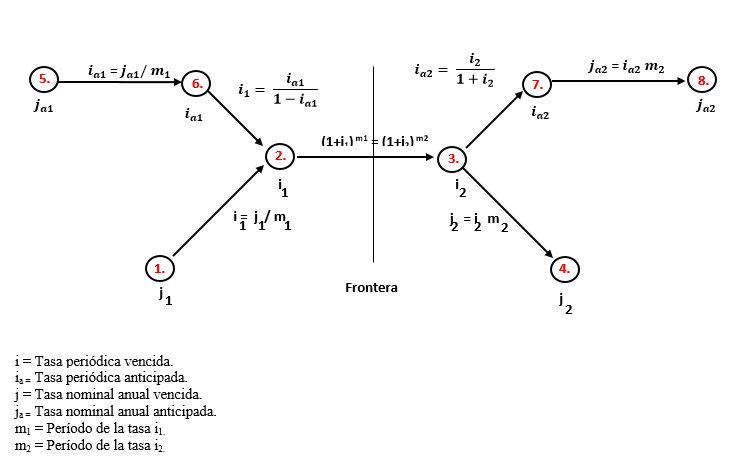
\includegraphics[height = 9.0 cm]{general}\\
\end{center}

Una tasa con período 200 días anticipada es representada con $i_{a}$.\\

Por lo tanto salimos del punto 5 y vamos al punto 4.\\

En el punto 6 $i_{a}$ = 20\% período  (200 días) anticipada.\\

En el punto 2- $i = \frac{i_{a}}{1-i_{a}} = \frac{0,2}{1-0,2} $= 0,25 p(200 días) a\\

Para ir del punto 2 al punto 3 debemos tener en cuenta que si un período tiene 200 días entonces en 1 año habrá $\frac{365}{200}$ períodos, de igual forma, si un período tiene 150 días en un año habrá $\frac{365}{150}$ períodos por tanto podemos plantear la siguiente ecuación:\\

$m_{1}= \frac{365dias}{200dias}$\\

$m_{2} = \frac{365dias}{150dias}$\\

$(1 + 0.25)^{\frac{365}{200)}} = (1 + i2)^{\frac{365}{150}}$\\


Para despejar la i es necesario deshacer el paréntesis de la derecha y para ello es necesario que quede elevado a la potencia 1, por tanto habrá que multiplicar los exponentes de la ecuación anterior por $\frac{150}{365}$, entonces la ecuación queda así:\\ 

$(1 + 0,25)^{\frac{365}{200}\frac{150}{365}} = (1+i)^{\frac{365}{150}\frac{150}{365}}$\\

$(1 + 0,25)^{\frac{150}{200}} = (1 + i)^1 $\\

1.1821770 = 1 + i\\

Despejando se tiene i=18.2177\% período 150 días que corresponde al punto 3.
Para llegar al punto 4 se aplica la formula j = i m\\

Entonces $j = 18.2177 x \frac{365}{150} = 44.33 \%na 150$dv\\

$j = 20\%\ (200dias)\ a\ \equiv 44.33\%na\ 150dv$

\section{Ecuaciones de valor}

Es muy frecuente cambiar una o varias obligaciones por otra u otras nuevas obligaciones. La solución de este problema es elemental y para solucionarlo es necesario usar ecuación de valor, que es una igualdad de valores ubicados en una sola fecha denominada fecha focal.\\

La fecha focal se representa gráficamente por una línea a trazos y por las letras ff y es la fecha en que debe hacerse la igualdad entre ingresos y egresos. La ubicación de la fecha focal no altera la respuesta final, por tal motivo la ubicación de la fecha focal se deja a libre elección de la persona que va a resolver el problema. (En interés simple, la posición de la fecha focal sí causa variación en la respuesta final y por esta razón normalmente es el acreedor quien decide donde ubicarla).\\

El principio fundamental de una ecuación de valor, que viene a ser el mismo principio fundamental de las finanzas, establece que la sumatoria de los ingresos debe ser igual a la sumatoria de los egresos ubicados ambos en la fecha focal, esto es:

\begin{center}
	$\sum ingresos = \sum egresos(en la ff)$\\
\end{center}
Naturalmente que el traslado a la fecha focal de cada una de las cantidades debe hacerse usando la fórmula del valor futuro o la fórmula del valor presente, segun el caso, utilizando una tasa de interés llamada el rendimiento normal del dinero que es la tasa que en promedio cobra el sistema financiero.\\

El enunciado de una ecuación de valor también puede ser expresado así:

\begin{center}
	$\sum deudas = \sum pagos(en la ff)$\\
\end{center}

Mirando un balance el principio puede ser expresado así:\\

\begin{center}
	$\sum activos = \sum pasivos + capital(en la ff)$\\
\end{center}

Como en cualquier proyecto los ingresos se representan por flechas hacia arriba y los egresos se representan por flechas hacia abajo entonces, mirando la gráfica de flujo de caja podemos expresar el principio fundamental de una ecuación de valor de esta otra forma:\\

\begin{center}
	$\sum de\ lo\ que\ esta\ para\ arriba = \sum de\ lo\ que\ esta\ para\ abajo(en\ la\ ff)$\\
\end{center}

La sumatoria de los ingresos en pesos de hoy menos la sumatoria de los egresos en pesos de hoy recibe el nombre de valor presente neto o valor actual neto (en la calculadora se representa por VAN y en EXCEL se representa por VNA).\\

La tasa a la cual la sumatoria de los ingresos es igual a la sumatoria de los egresos se denomina tasa interna de retorno que en el texto se representará por TIR.\\

En capitulo posterior analizaremos más en detalle los conceptos de VPN: valor presente neto y TIR, estos conceptos son de suma importancia en la evaluacion de proyectos.\\

\textbf{Ejemplo 20}\\

Una persona se comprometió a pagar \$250.000 en 3 meses, \$300.000 en 8 meses y \$130.000 en 15 meses. Ante la dificultad de cumplir con las obligaciones tal como están pactadas solicita una nueva forma de pago así: \$60.000 hoy, \$500.000 en 12 meses y el saldo en 18 meses. Suponiendo que el rendimiento normal de la moneda es del 36\% nominal anual mes vencido, determinar el valor del saldo.\\

\begin{itemize}
	\item a. Diagrama de flujo de caja.\\
	\begin{center}
		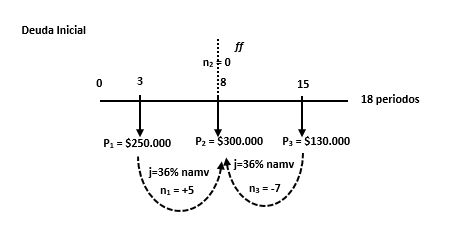
\includegraphics[height = 6.0 cm]{2_17_1}\\
	\end{center}
	
	\begin{center}
		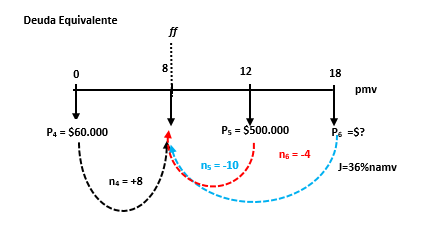
\includegraphics[height =6 cm]{2_17_2}\\
	\end{center}
	
	\item b. Declaración de variables:\\
	
	
	$j = 36\%namv$
	\\$ i = \frac{36\%}{12}$pmv = 3\% pmv
	\\
	$P_{1} = \$250.000; \hspace{35 pt}$n_{1} = +5 pmv;\\
	P_{2} = \$300.000;$\hspace{37 pt}n_{2} = 0 $ pmv\\
	P_{3} = \$130.000$; \hspace{30 pt} 	$n_{3} = -7 pmv;\\
	$P_{4} = \$60.000; \hspace{40 pt}n_{4} = +8 $ pmv;\\
	P_{5} = \$500.000$; \hspace{32 pt}	$n_{5} = -4 pmv;\\ \\ P$_{6}$=\$?\\ 
	n_{6} = -10 $ pmv;\\
	   Fecha focal (ff): en el mes 8.\\    
  	
	
	\item c. Declaración de fórmulas:\\
	
	$F = P(1+i)^n$ \hspace{35 pt} \textit{Valor futuro dado un valor presente}\\
	$P = F(1 +i)^{-n}$\hspace{33 pt} \textit{Valor presente dado un valor futuro}\\
	
	\item d. Procedimiento matemático\\
	
	$F_{1} + F_{2} + P_{3} = F_{4} + P_{5} + P_{6}$ \hspace{35 pt}\textit{Ecuacion de valor.}\\
	
	La ecuación de valor puede ser escrita, en la fecha focal ff 8 para el período octavo, así:\\
	
	$\$250.000(1+0,03)^5 + \$300.000(1+0,03)^0 + \$130.000(1+0,03)^{-7} = \$60.000(1+0,03)^8 + \$500.000(1+0,03)^{-4} + P_{6}(1+0,03)^{-10}$\hspace{33 pt} \textit{Ecuación de valor}\\
	
	Al despejar 	$P_{6}$ de esta ecuación se tiene:
	
	$P_{6} = \$235.549.16$\\
	
	\item e. Respuesta:\\
	
	La solución será: $P_{6}$ = \$235,549.16\\
	
	
\end{itemize}

\textbf{Ejemplo 21}\\

Una deuda de \$15.000 fue contraída hace 2 meses con fecha de vencimiento en 4 meses, esta posee un interés del 24\% nominal anual trimestre vencido y otra deuda de \$25.000 contraída hace un mes con vencimiento de 8 meses e intereses del 28\% nominal anual semestre vencido, se van a cancelar mediante dos pagos de igual valor, efectuados el primero el día de hoy y el segundo en 6 meses. Con un interés del 30\% nominal anual mes vencido y el segundo en 6 meses, con un interés del 30\% nominal anual mes vencido, determinar el valor de los pagos.\\

\begin{itemize}
	\item a. Diagrama de flujo de caja:
	\begin{center}
		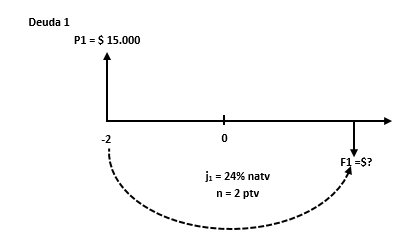
\includegraphics[height = 6.0 cm]{2_18_1}\\
	\end{center}
	
	\begin{center}
		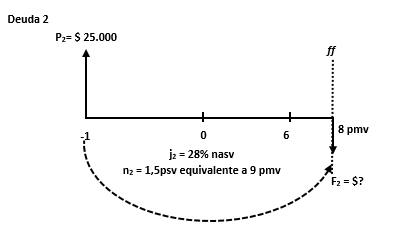
\includegraphics[height = 7.0 cm]{2_18_2}\\
	\end{center}
	
		\begin{center}
		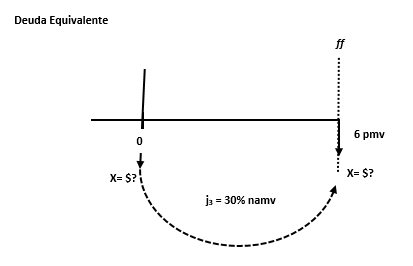
\includegraphics[height = 7.0 cm]{2_18_3}\\
	\end{center}
	
	\item b. Declaración de variables:\\
	
	Deuda 1:\\
	$j_{1}$ = 24\% natv\\	
	$i_{1}$ = 6\% ptv\\	
	$n_{1}$ = 2 ptv\\
	
	$P_{1}$ = \$15.000    \\
    $F_{1}$ = \$?
	
	Deuda 2\hspace{5 pt}:\\
	
	$j_{2}$ = 28\% nasv\\	
	$i_{2}$ = 14 \% psv\\	
	$n_{2}$ = 1,5 psv 
	
	$P_{2}$ = \$25.000   \\ 
    $F_{2}$ = \$? \\
	
	Deuda equivalente:\\
	
	$j_{3}$ = 30\% namv\\	
	$i_{3}$  = 2.5\% pmv\\
	
	$ff$ = fecha focal: mes 6\\
    
    $P_{3} = F1$\\    
    $F_{3} = F2$\\
    
	
	\item c. Declaración de fórmulas:\\
	
	$F = P(1+i)^n$\hspace{35 pt} \textit{Valor futuro dado un valor presente}\\
	$P = F(1+i)^{-n}$\hspace{35 pt} \textit{Valor presente dado un valor futuro}\\
	
	\item d. Procedimiento matemático:\\
	
	Primero debemos liquidar el valor de cada deuda en la fecha de su vencimiento\\
	
	$F_{1} = \$15.000(1 + 0,06)^2 = \$16.854$\\
	$F_{2} = \$25.000(1 + 0,14)^{1.5} = \$30.429,67$\\
	
	A continuación el planteamiento de la ecuación de valor será:\\ 
	
	\$ 16.854(1 +0,025)^2 + \$30.429,67(1 + 0,025)^{-2} = X(1 + 0,025)^6 + X$ \hspace{35}\textit{Ecuación de valor}\\
	
	\item e. Respuesta:\\
	
	La solución será: X = \$21.609,84\\
	
	
\end{itemize}

\textbf{Ejemplo 22}\\

Una persona debe pagar \$10.000 con vencimiento en 3 meses, \$15.000 a 10 meses y \$20.000 con vencimiento en un año. Si hace un pago único de \$45.000, hallar la fecha en que debe hacerse, suponga una tasa del 18\% nominal anual mes vencido.\\
Si consideramos la fecha focal (ff) en el mes 12:\\

\begin{itemize}
	\item a. Diagrama de flujo de caja:\\
	\begin{center}
		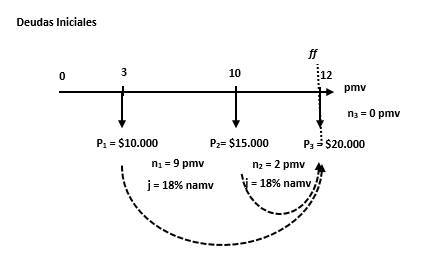
\includegraphics[height = 6.0 cm]{2_19_1}\\
	\end{center}
	
	\begin{center}
		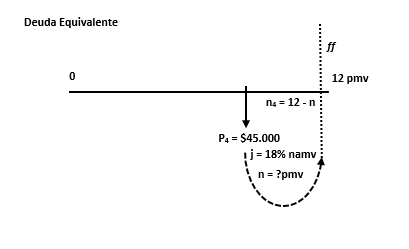
\includegraphics[height = 5.5 cm]{2_19_2}\\
	\end{center}
	
	\item b. Declaración de variables:\\
	$j$ = 18\% namv\\ i = 1,5\%pmv\\
	
	$P_{1} = \$10.000; \hspace{35 pt}$n_{1}$ = +9pmv ;\\ P_{2} = \$15.000; \hspace{35 pt}$n_{2} = 2$ pmv\\
	
 $P_{3} = \$20.000$ \hspace{35 pt}	$n_{3}$ = 0 pmv \\  $P_{4} = \$45.000$ \hspace{35 pt} $n_{4}$ =12-n$\\
	
	
	
	\item c. Declaración de fórmulas:\\
	
	$F = P(1+i)^n$ \hspace{35 pt} \textit{Valor futuro }\\
	$P = F(1+i)^{-n}$ \hspace{35 pt} \textit{Valor presente}\\
	
	\item d. Procedimiento matemático:\\
	
	El planteamiento de la ecuación de valor será:\\
	
	$\$10.000(1+0,15)^9 + \$15.000(1 + 0.015)^2 + \$20.000(1 + 0,015)^0 = \$45.000(1+0.015)^{12-n}$ \hspace{35 pt} \textit{Ecuacion de valor}\\ 
	
	$\$46.887,27 = \$45.000(1,015)^{12-n}$\\
	
	$\frac{\$46.887,27}{\$45.000} = (1,015)^{12-n}$\\
	
	$1,00419394 = (1,015)^{12-n}$\\
	
	$log1,00419394= (12-n)log1,015$\\
	
	$(12 - n) = \frac{log1,00419394}{log1,015}$\\
	
	$(12 - n) = 2,759409869$\\
	
	$n = 9,240959 pm$\\
	
	\item e. Respuesta:\\
	
	El pago único de \$45.000 lo debe hacer a los 9,240959 meses.\\
	
	En la respuesta anterior existen 9 meses + 0,24059 de mes, y mediante una proporción se puede establecer el número de días que hay en la fracción de mes así:\\
	Un mes tiene 30 días, en 0,24059 de mes, ¿Cuántos días hay?\\
	
\begin{table}[]
\centering
\label{my-label}
\begin{tabular}{|c|c|}
\hline
\textbf{MES} & \textbf{DÍAS} \\ \hline
1            & 30            \\ \hline
0,24         & x             \\ \hline
\end{tabular}
\end{table}

	Despejando se tiene que X = 7,2177 días.\\
	
	La fecha exacta sería 9 meses con 7,2177 días.\\
	
\end{itemize}

\textbf{Ejemplo 23}\\

Una persona debe pagar \$70.000 en 3 meses y \$85.000 en 8 meses; ante la imposibilidad de cancelar las deudas en las fechas previstas le ofrece al acreedor que le cancelara \$50.000 en 4 meses y \$130.000 en 12 meses. Si el acreedor acepta esta nueva forma de pago ¿Qué tasa de interés periódica mes vencido estará pagando?\\

\begin{itemize}
	\item a. Diagrama de flujo de caja:\\
	
	\begin{center}
		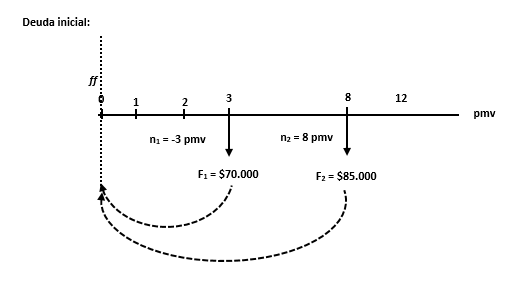
\includegraphics[height = 6.0 cm]{2_21_1}\\
	\end{center}
	
	\begin{center}
		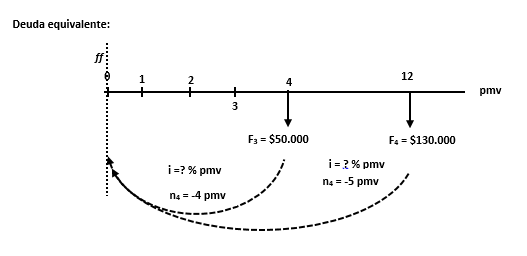
\includegraphics[height = 6.0 cm]{2_21_2}\\
	\end{center}
	
	\item b.Declaración de variables:\\
	
	i=?\% pmv\\
	$F_{1} = \$70.000$ ; \hspace{25}$n1 = -3$ pmv\\
    $F_{2} = \$ 85.000$; \hspace{25}$n2 = -8$pmv \\
    $F_{3} = \$ 50.000$; \hspace{25}$n3 = -4$ pmv\\
    $F_{4} = \$130.000$; \hspace{22}$n4= -12$pmv \\
	
	\item c. Declaración de fórmulas:\\
	
	$F = P(1 + i)^n$ \hspace{35}\textit{Valor futuro}\\
	$P = F(1 + i)^{-n}$\hspace{35}\textit{Valor presente}\\
	$P_{1} + P_{2} = P_{3} + P_{4}$\hspace{35}\textit{Ecuación de valor}\\
	
	\item d. Procedimiento matemático:\\
	
	La incógnita es la tasa i, en consecuencia el planteo de la ecuación de valor será:\\ \\
	$\$70.000(1+i)^{-3}+\$85.000(1+i)^{-8} = \$50.000(1+i)^{-4} + \$130.000(1+i)^{-12}$
	
	El procedimiento para resolver este problema de forma manual es el siguiente:\\
	
	\begin{itemize}
		\item Se iguala toda la ecuación a cero, y se simplifica por mil:\\
		
		$70(1 + i)^{-3} + 85(1 + i)^{-8} - 50(1 + i)^{-4} - 130(1 + i)^{-12} = 0$\\
		
		\item  Para resolver esta ecuación utilizaremos el método de ensayo y error combinado con una interpolación, el método consiste en escoger una tasa $i_{1}$ y calcular el valor que toma la función $f_{1}$, luego haremos lo mismo con una tasa $i_{2}$ y calculamos el valor que toma la función $f_{2}$, lo importante es que el valor de las funciones $f_{1} y f_{2}$ sean de signo diferente, si al hacer los ensayos las funciones salen del mismo signo, habrá que hacer nuevos ensayos hasta que obtengamos las funciones con signo diferente.\\
		
		\item 	De acuerdo a lo anterior hacemos un primer ensayo con $i_{1}$ = 2\% pmv , entonces al remplazar en la ecuación esta ya no va a ser igual a 0 y su resultado será:\\
		
		$70(1 + 0,02)^{-3} + 85(1 + 0,02)^{-8} - 50(1 + 0,02)^{-4} - 130(1 + 0,02)^{-12} = -10,18714$\\
		
		\item 	Ahora procederemos con el ensayo de $i_{2} =3\% pmv$ y la ecuación con su resultado será:\\
		
		$70(1 + 0,03)^{-3} + 85(1 + 0,03)^{-8} - 50(1 + 0,03)^{-4} - 130(1 + 0,03)^{-12} = -4,44404$\\
		
		\item Como el valor de la función en ambos casos es negativo entonces tenemos que hacer un nuevo intento con otra tasa de interés hasta que cambie de signo, por eso ensayamos con $i_{3} = 4\%$ pmv y la ecuación será:\\
		
		$70(1 + 0,04)^{-3} + 85(1 + 0,04)^{-8} - 50(1 + 0,04)^{-4} - 130(1 + 0,04)^{-12} = -0,40058$\\
		
		\item Tomamos los resultados correspondientes al 3\% y a 4\% por ser los más cercanos y los que presentan diferente signo y los colocaremos de la siguiente forma:\\
		
		\begin{center}
			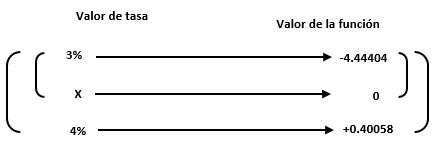
\includegraphics[height = 3.0 cm]{2_22}\\
		\end{center}
		
		\item Ahora planteamos una proporción, teniendo en cuenta las diferencias mostradas en los corchetes y siempre manteniendo el mismo orden, por ejemplo: la diferencia pequeña es a la diferencia grande del lado izquierdo igual que la diferencia pequeña es a la diferencia grande del lado de la derecha.\\
		
		\begin{center}
			$\frac{3-i}{3-4} = \frac{-4.44404 - 0}{-4.44404 - 0.40058}$\\
		\end{center}
		
		
		
	\end{itemize}
	
	\item e. Respuesta:\\
	
	Al despejar i de la ecuación anterior tenemos: i= 3,91735 pmv.\\
	
\end{itemize}

\textbf{Observación:} La interpolación produce un error que es despreciable siempre y cuando el intervalo que se toma para interpolar no sea muy grande, en la práctica financiera un punto porcentual es el máximo permitido para que el error sea despreciable, en este caso hemos usado un punto porcentual porque hemos interpolado entre el 3\% y el 4\%. La respuesta exacta con 7 decimales es: 3.9104765\% pmv.



\cleardoublepage
\phantomsection
\setlength{\columnsep}{0.75cm}
\printindex
